\section{Results and discussion}
% Define a custom command to create sections with shared structure

As explained in \autoref{sec:methodo}, the first objective is to effectively post-process a single NWP forecast model, by benchmarking the models altogether. 

The following step will be to look at the results in the details to prove the true effectiveness of the post-processing.

We will each time first study the MAE optimisation and then the RMSE optimisation. Be aware that the models hyperparameters may vary between the two optimisations because the 
target metrics to minimize is not the same during the computations.
\subsection{Post-processing of a single forecasting NWP model}
\subsubsection{Study of the post-processing models altogether} \label{subsubsec:pp}
\paragraph{MAE}\indent
\begin{figure}[htb!]
    \centering
    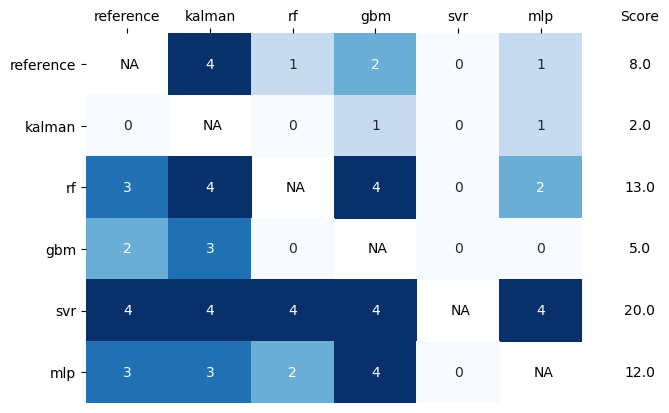
\includegraphics[width=\columnwidth]{figures/first_study/significance_matrix_mae.png}
\caption{Significance matrix for MAE. The value $V_{(i,j)}$ of the $(i,j)$ cell indicates how often the model of line i performs better than the one of column j, across the 
4 sites. For example, the MAE of the MLP model post-processed data is 3 times lower than the MAE of the reference model, and for 1 site (4 - 3 = 1), it is higher.}
\label{fig:sig_mae}
\end{figure}

\begin{figure}[htb!]
    \centering
    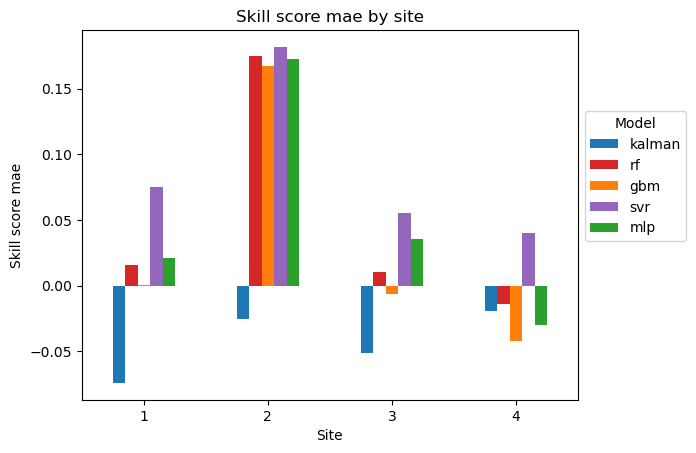
\includegraphics[width=\columnwidth]{figures/first_study/ss_mae.png}
    \caption{MAE skill score plot across the 4 sites.}
\label{fig:ss_mae}
\end{figure}
\autoref{fig:sig_mae} clearly shows that the SVR model is the best one for MAE. It performs better than any of the other model on any of the 4 study cases.

\autoref{fig:ss_mae} demonstrates that the sites 1, 3 and 4 heavily benefit from this model with respect to the other ones. 
On site 4, the only positive post-processing is given by the SVR model.

The Kalman filter showcases really poor performances across the 4 sites.

\newpage
\paragraph{RMSE}\indent

\begin{figure}[htb!]
    \centering
    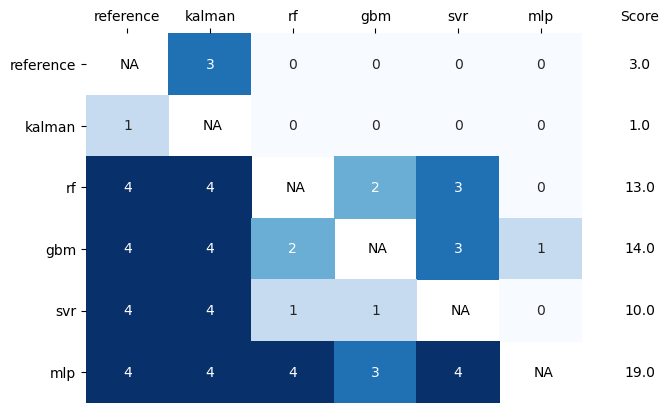
\includegraphics[width=\columnwidth]{figures/first_study/significance_matrix_rmse.png}
\caption{Significance matrix for RMSE. The value $V_{(i,j)}$ of the $(i,j)$ cell indicates how often the model of line i performs better than the one of column j, across the 
4 sites. For example, the RMSE of the MLP model post-processed data is 3 times lower than the RMSE of the reference model, and for 1 site (4 - 3 = 1), it is higher.}
\label{fig:sig_rmse}
\end{figure}

\begin{figure}[htb!]
    \centering
    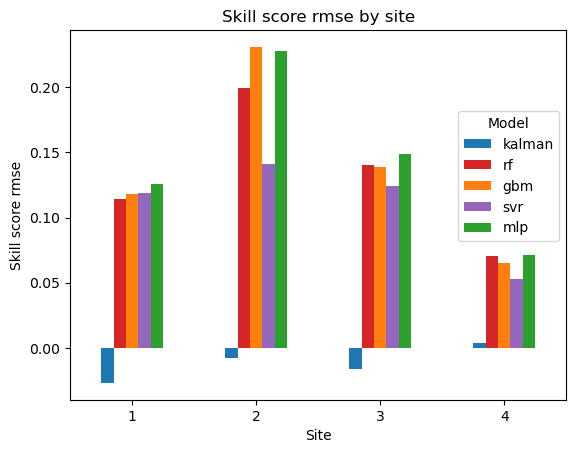
\includegraphics[width=0.5\columnwidth]{figures/first_study/ss_rmse.png}
    \caption{RMSE skill score plot across the 4 sites.}
    \label{fig:ss_rmse}
\end{figure}

The results of the RMSE are not the same, and it is the MLP model that performs the best, achieving the highest score in the matrix of \autoref{fig:sig_rmse}.

This is confirmed by \autoref{fig:ss_rmse} where the MLP model bar is the highest for 3 sites out of 4.

\newpage
\subsubsection{Detailled study of the most performing model}
With the aim of clarity, only the plots of the single site 2 will be shown here.
The overall similarity of the results across the 4 sites also motivate this choice.

The ones of the other sites can be found in \autoref{appendix:single} to fortify the belief in the analysis drawn for a single site.

\paragraph{MAE}\indent
\begin{figure}[htb!]
    \centering
    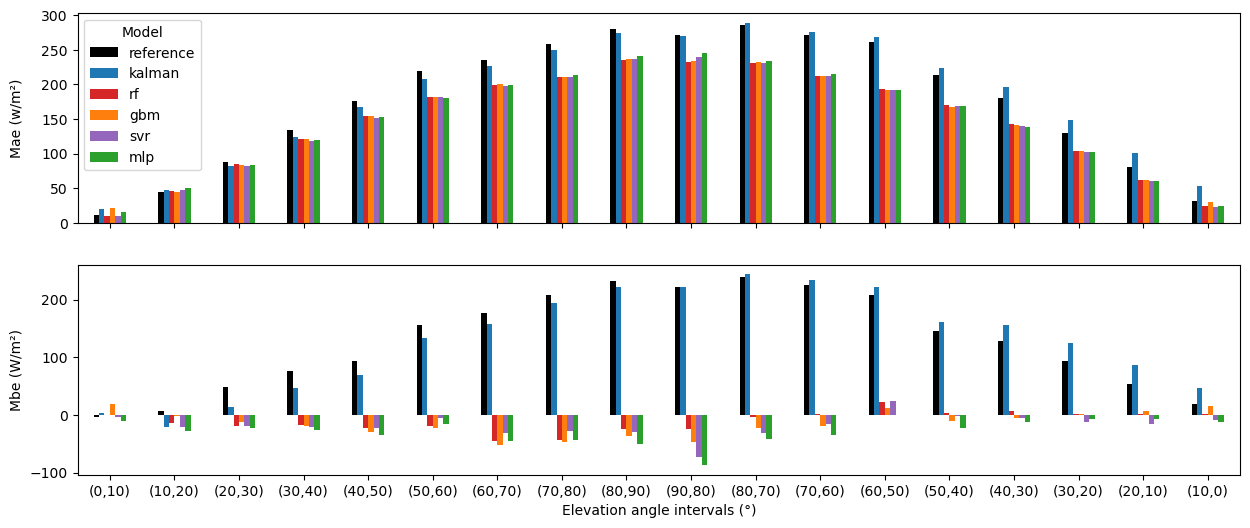
\includegraphics[width=1.1\columnwidth]{figures/first_study/mae_mbe_site2.png}
\caption{MAE and MBE levels across all elevation angle intervals of a day, for site 2.}
\label{fig:mae_mbe_site2}
\end{figure}

    \autoref{fig:mae_mbe_site2} supports our previous conclusions, but most importantly shows the decrease of the MBE across all the elevation angle intervals of a day.
Indeed, it is a know fact that NWP models present a positive bias that is higher around noon, and the MBE of all the machine learning models tends to be much closer to 0.

On site 2, the bias is negative but this bias can be either positive or negative depending on the study site, as confirmed with the other graphs in \autoref{appendix:single}.

Only site 4 shows a different behavior for the bias across the day, even if the MAE is improved. 
\begin{figure}[htb!]
    \centering
    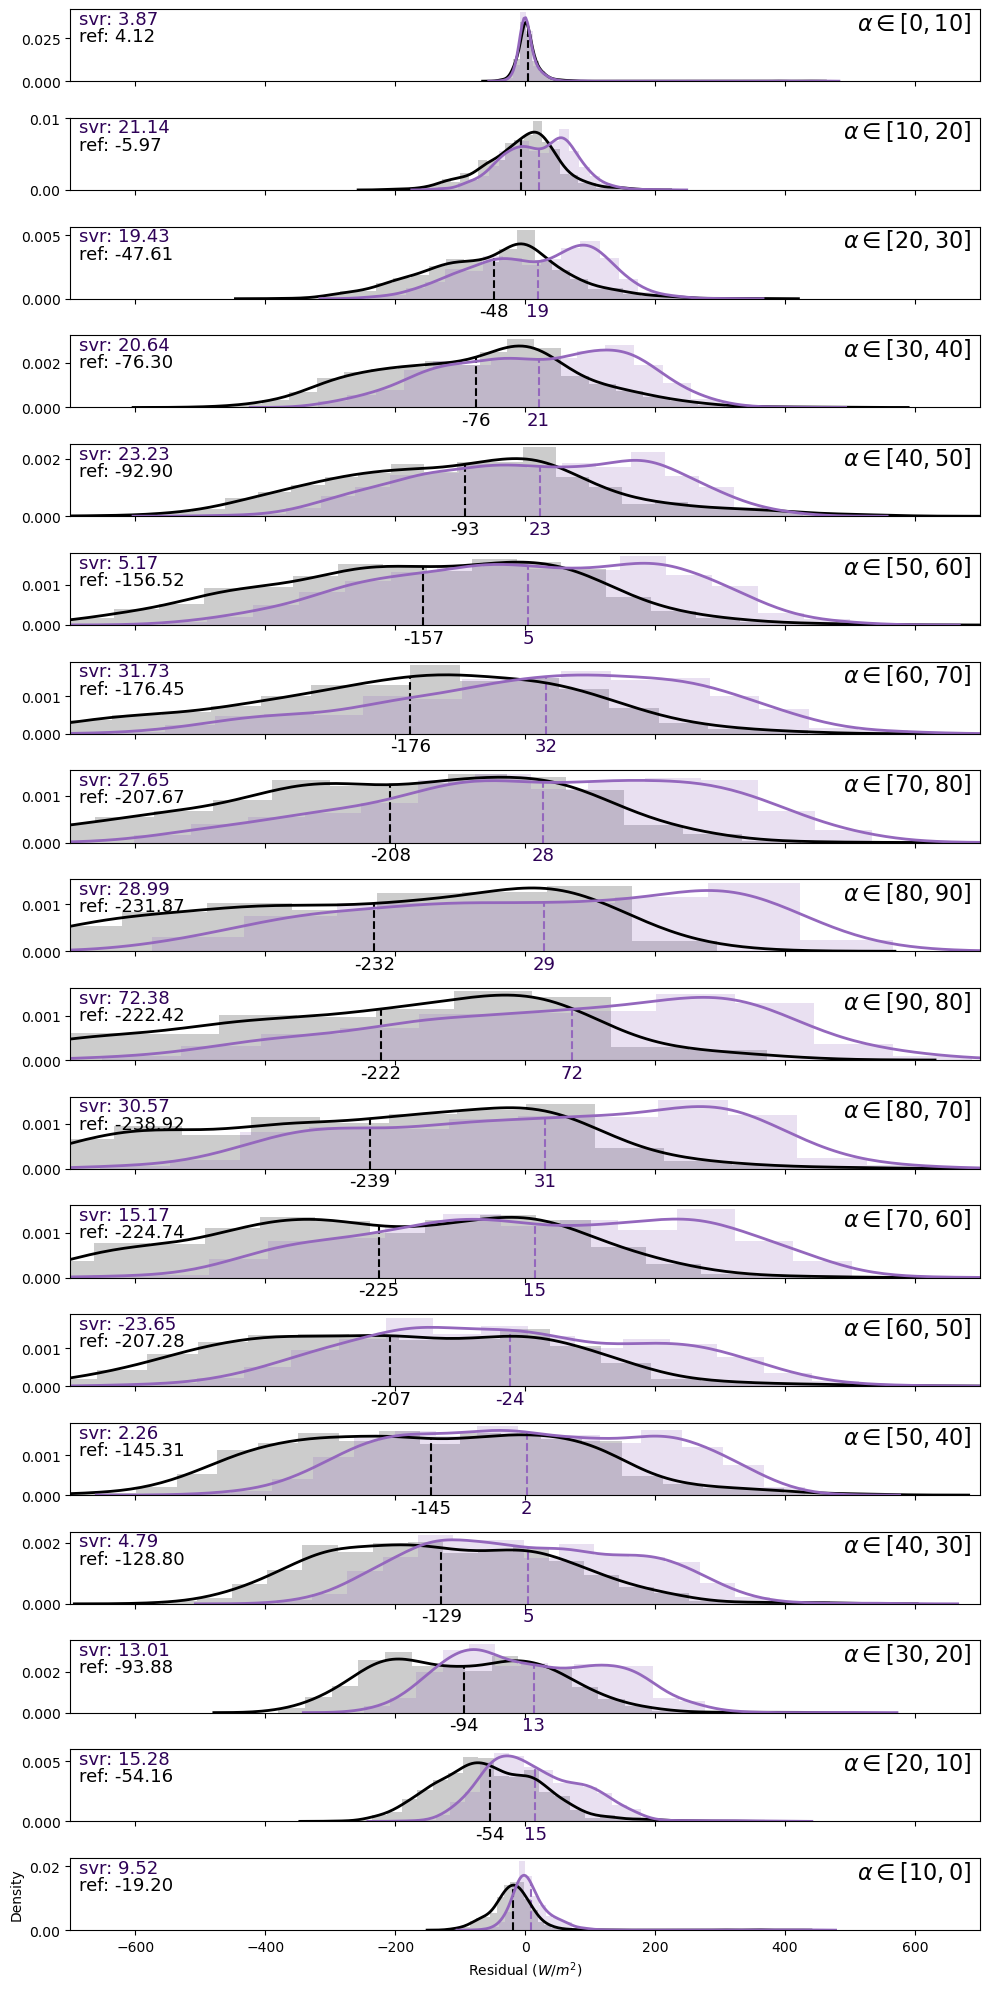
\includegraphics[width=0.47\columnwidth]{figures/first_study/residual_errors_svr_site2_mae.png}
\caption{Residual error levels across all elevation angle intervals of a day, for a SVR model, for site 2.}
\end{figure}

The probability density functions across the day support these conclusions, where we can clearly see that the curves means are shifted toward 0, as are the scatter plots in \autoref{appendix:single}.
The whole dataset cloud is shifted towards the line y=x, which is the line where the corrected forecast exactly match the measured irradiance.
This shift does not depend of the sign of the initial bias, since even positive mean biases occuring at late hours for site 4 are effectively shifted to the left. \\

These plots of the MAE minimisation with the SVR model show that this model is not only able to reduce the MAE across the day, but also to reduce the MBE across the day.

The global lowering of the metrics is indeed reflected in the lowering of the metrics at each elevation angle interval of particular day. The bias is also improved in 3 sites out of 4.
\paragraph{RMSE}\indent

Similar conclusions can be drawn about the RMSE minimisation, with the MLP model.

The only difference is that the improvement of the MBE now stands for all the study cases.

\begin{figure}[htb!]
    \centering
    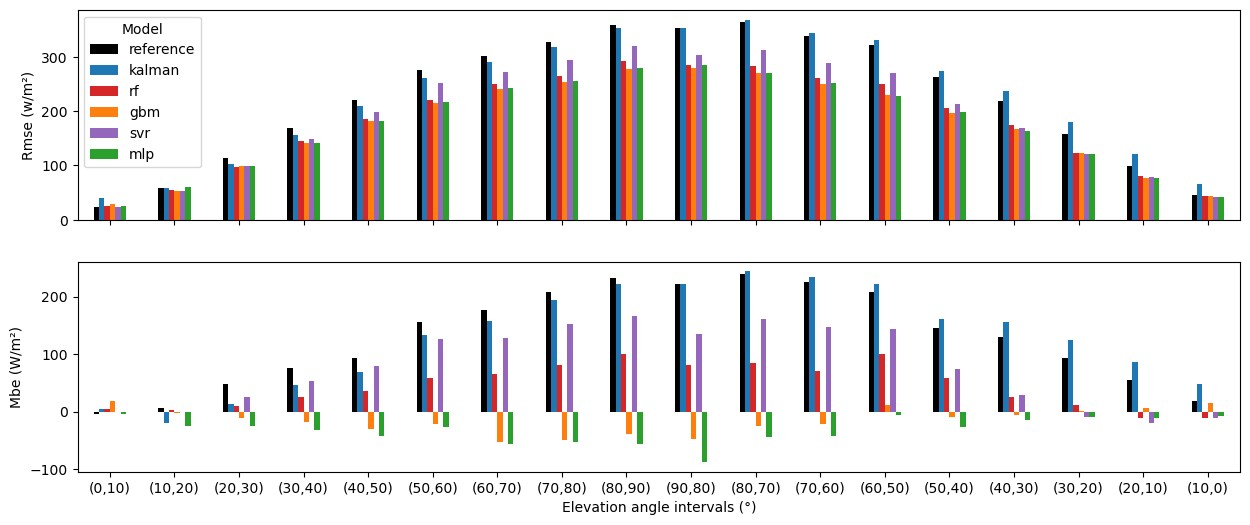
\includegraphics[width=\columnwidth]{figures/first_study/rmse_mbe_site2.png}
\caption{RMSE and MBE levels across all elevation angle intervals of a day, for site 2.}
\end{figure}
\newpage

\begin{figure}[htb!]
    \centering
    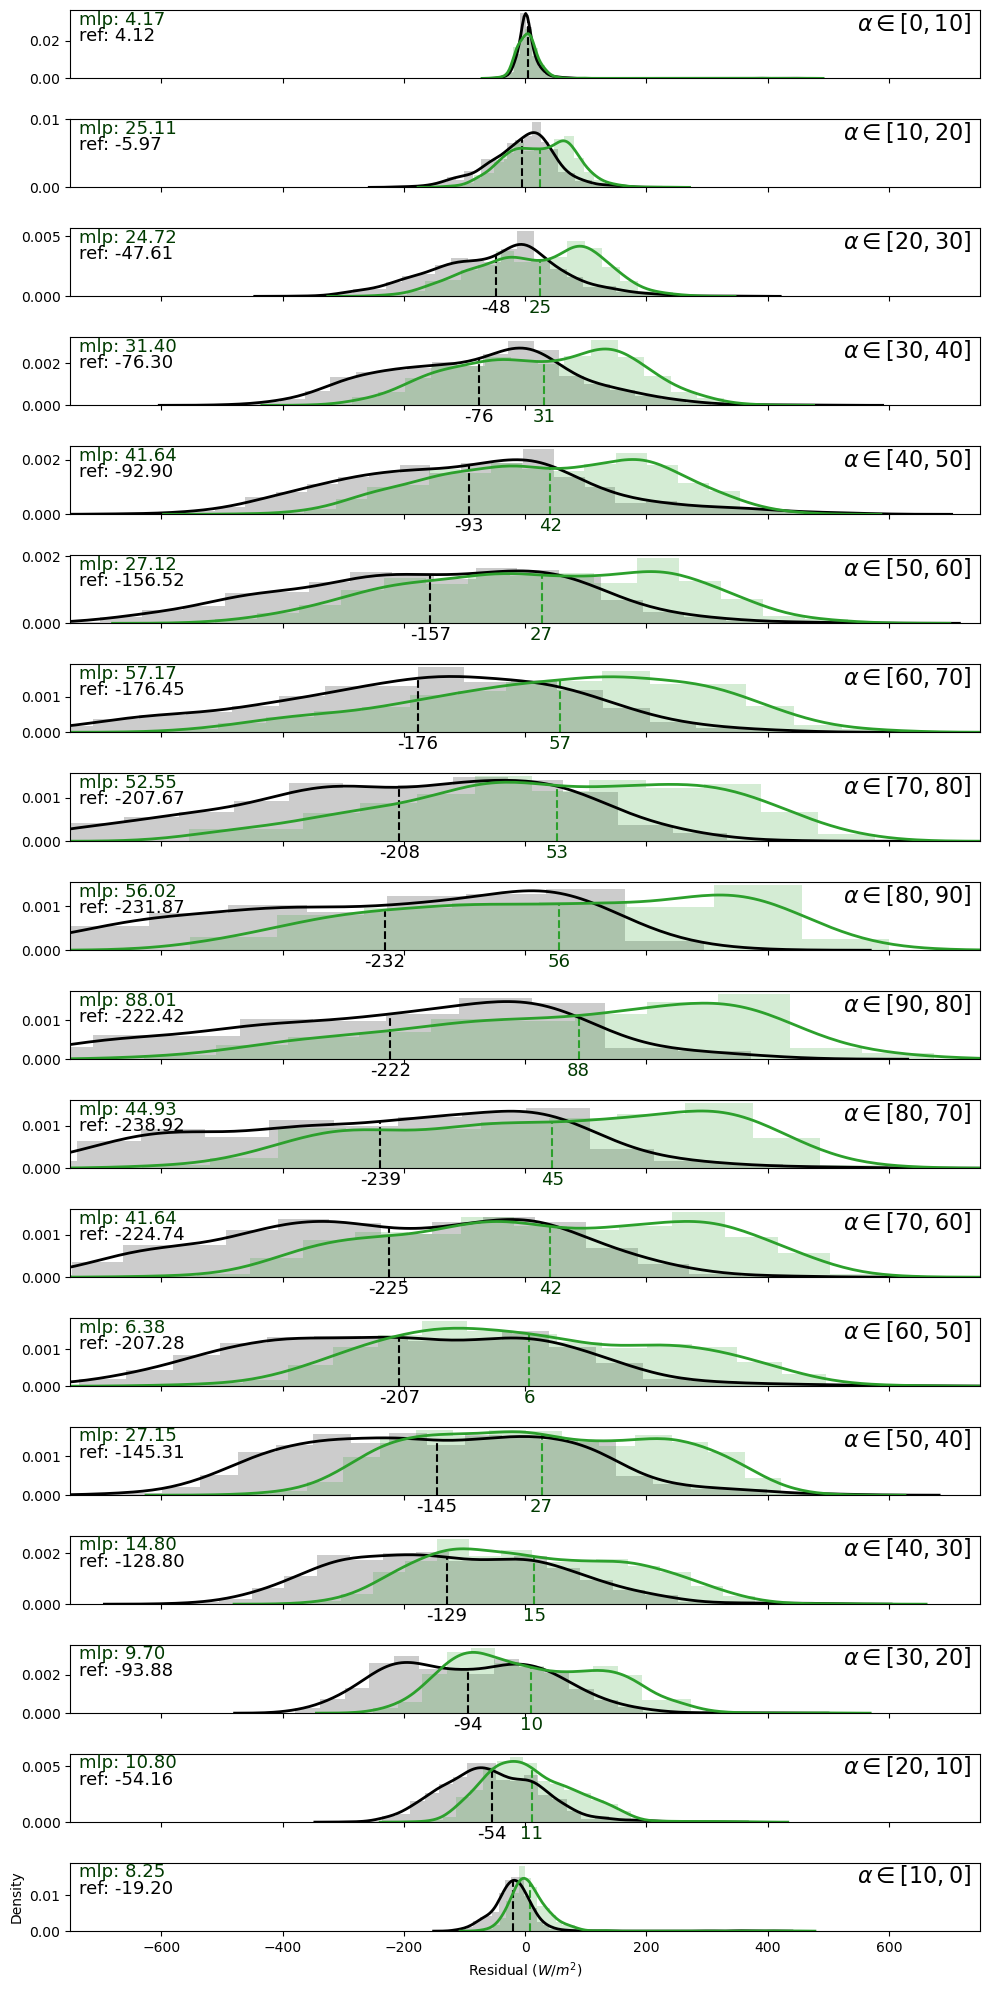
\includegraphics[width=0.47\columnwidth]{figures/first_study/residual_errors_mlp_site2_rmse.png}
\caption{Residual error levels across all elevation angle intervals of a day, for a MLP model, for site 2.}
\end{figure}

All in all, the improvement of the metrics of interest (MAE and RMSE) is reflected in an improvement of the bias. 

This behavior stands for each period of a day, which was not perfectly obvious after I performed the global post-processing.\\

Once the relevant models have been found, one has to perform a sensitivity study of these ones in order to better grasp how they work.

\subsubsection{Sensitivity study}
A sensitivity study of the parameters that are not tuned in our process has to be performed. It is why the influence of the choices of predictors, of learning periods, of learning window type (fixed or sliding) and of forecasting model are successively studied. 

With the aim of clarity, the results will be here presented with the MAE optimisation, but the results of the RMSE optimisation lead the same conclusions, and can also
be found in \autoref{appendix:single}.

It's important to notice that for each sensitivity study, only the one parameter investigated is modified from the framework defined in \autoref{sec:methodo}, all the rest is kept constant.

\paragraph{Influence of the choice of the predictors}
\indent

The first sensitivity study is performed with the set of predictors that was presented in \autoref{tab:set_pred}, and the different configurations are described in \autoref{tab:pred_configs}.
\begin{table}[htb!]
\begin{center}
\begin{tabular}{|l|llll|}
\toprule
{} &  0 &  1 &  2 &  3 \\
\midrule
$ghi_{GFS}$            &  X &  X &  X &  X \\
$temperature^{2m}_{GFS}$ &  X &  X &    &    \\
$\theta$             &  X &  X &  X &    \\
$\phi$            &  X &  X &  X &    \\
$ghi_{cs}$             &  X &    &  X &    \\
\bottomrule
\end{tabular}
\end{center}
\label{tab:pred_configs}
\caption{Description of the configurations of the sets of predictors.}
\end{table}

\newpage
\begin{figure}[htb!]
    \centering
    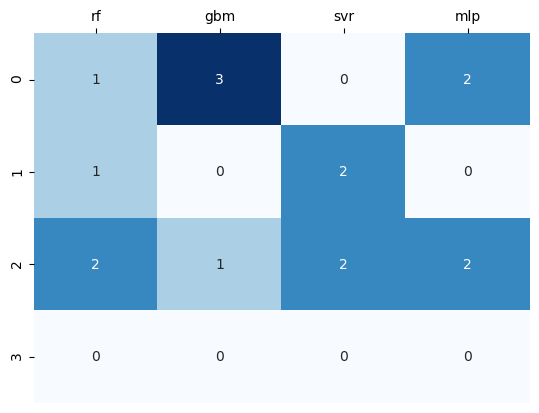
\includegraphics[width=0.6\columnwidth]{figures/first_study/comp_predictors_mae.png}
\caption{Pairwise systematicity matrix for MAE. The value $V_{i,j}$ of the cell $(i,j)$ indicates how often the configuration of line i is the best one, across the 4 sites, for the model of column j. For example, the configuration 0 is the best one with a GBM post-processing for 3 sites, and the configuration 2 is the best one for 1 site.}
\label{fig:matrix_pred}
\end{figure}

\begin{figure}[htb!]
    \centering
    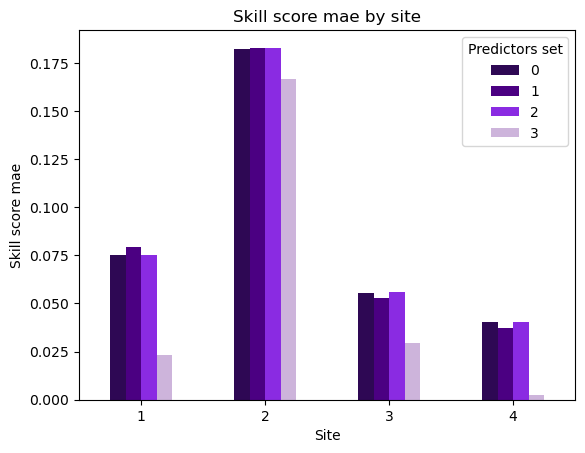
\includegraphics[width=0.72\columnwidth]{figures/first_study/comp_predictors_mae_svr.png}
\caption{Comparison of the MAE skill scores of the different configurations.}
    \label{fig:ss_pred}
\end{figure}

\newpage
Interestingly, the configuration with all the predictors is not the configuration that seem to give the best results if we consider \autoref{fig:matrix_pred}.

If we consider now \autoref{fig:ss_pred}, the performances of the configurations 0, 1 and 2 are nearly identical. They both provide great improvements to the post-processing using only the forecasted irradiance.

In the following, I chose to always rely on the full configuration of the set of predictors. This is because I was working with only 5 predicting values and a feature selection is generally not advised when working with so few predictors.
This is a strong choice that could be questioned if the situation were to work with much more predictors (more than 10), where a feature selection would be necessary, both for metrics and computational performances reasons.
\paragraph{Influence of the learning period}
\indent
\begin{figure}[htb!]
    \centering
    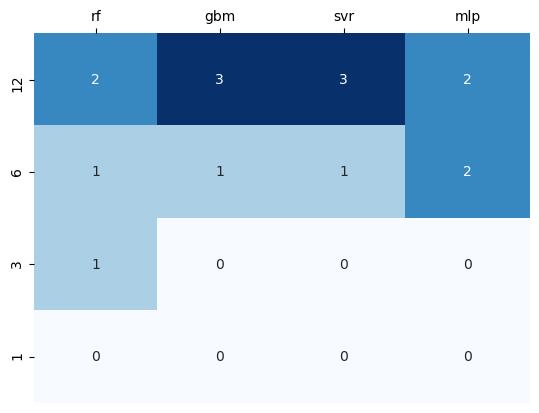
\includegraphics[width=0.7\columnwidth]{figures/first_study/comp_learning_period_mae.png}
\caption{Pairwise systematicity matrix for MAE. The value $V_{i,j}$ of the cell $(i,j)$ indicates how often the learning period duration (in months) of line i performs the best, across the 4 sites, for the model of column j. For example, having a 12-months-long learning period is the best thing in 3 sites out of 4 with a SVR model, the last site performs better with a 6-month-long learning period.}
\label{fig:matrix_period}
\end{figure}

\newpage
\begin{figure}[htb!]
    \centering
    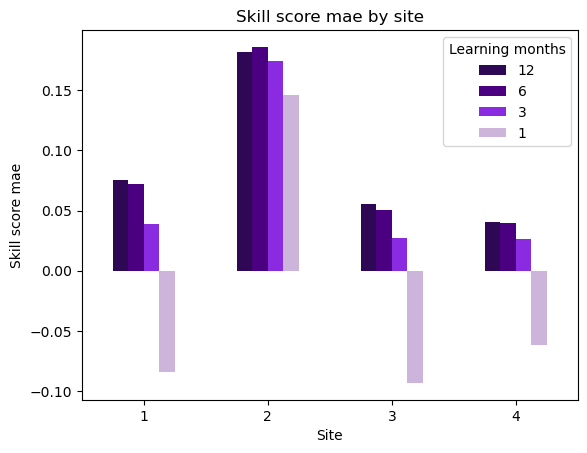
\includegraphics[width=0.70\columnwidth]{figures/first_study/comp_learning_period_mae_svr.png}
\caption{Comparison of the MAE skill scores of the different learning period durations (in months).}
    \label{fig:ss_period}
\end{figure}

Both \autoref{fig:matrix_period} and \autoref{fig:ss_period} go to show that a larger learning period is beneficial for the model, up to one year when 
the benefits from increasing the learning period do not prove to be significant.

It is interesting to notice that a one-month learning period provides a negative post-processing.
\paragraph{Influence of the learning window}
\indent 

Another question from Reuniwatt was the pertinence of a sliding learning window.

I thus performed two types of learning:
\begin{itemize}
    \item A fixed window learning where the testing period was the full year of 2021 and and the learning period was the full year of 2020.
    \item A sliding window learning where each month of the test year 2021 used a model trained during the moving year that preceded this month. For instance, March 2021 used a model trained from February 2020 to February 2021.
\end{itemize}
\newpage
\begin{figure}[htb!]
    \centering
    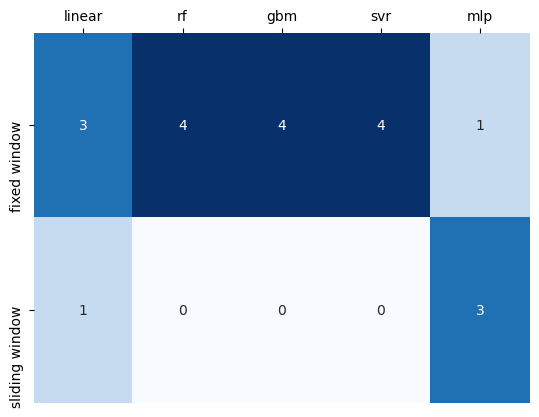
\includegraphics[width=0.7\columnwidth]{figures/first_study/comp_window_mae.png}
\caption{Pairwise systematicity matrix concerning window type for MAE.}
\end{figure}

\begin{figure}[htb!]
    \centering
    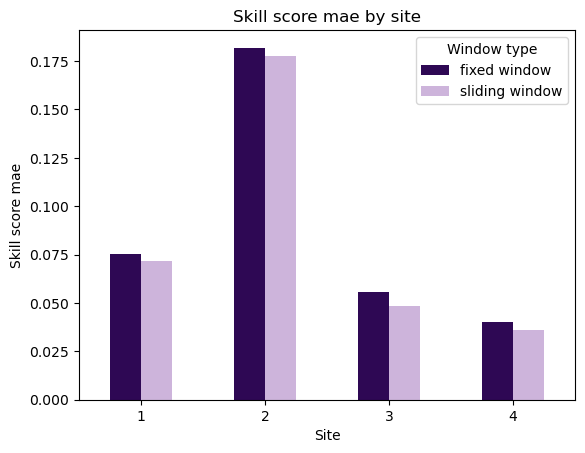
\includegraphics[width=0.72\columnwidth]{figures/first_study/comp_window_mae_svr.png}
\caption{Comparison of the MAE skill scores for a SVR model.}
\end{figure}

Interestingly, the fixed window performs best that the sliding window for all the study cases, even if the difference is nearly negligible.

\paragraph{Influence of the NWP forecasting model}
\indent

All the previous optimisations were done on the GFS forecast, as it was explained in \autoref{sec:methodo}.

Reuniwatt uses the data from several different (NWP) models, including ECMWF, AROME and ARPEGE.
It is interesting to see how our models perform on these different data sources.
\begin{figure}[htb!]
    \centering
    \includesvg[width=\columnwidth]{figures/first_study/comp_for_models_ss_mae.svg}
    \caption{Comparison of the MAE skill scores of the SVR model of four different NWP forecast models.}
    \label{fig:models_ss}   
\end{figure}
\newpage
\begin{figure}[htb!]
    \centering
    \includesvg[width=0.9\columnwidth]{figures/first_study/comp_for_models_mae.svg}
\caption{Comparison of the post-processing of four different NWP forecast models on MAE.}
\label{fig:models_plot}
\end{figure}

\autoref{fig:models_ss} clearly shows that the NWP models differently benefit from the post-processing.
There seems to be higher skill scores for less elaborate models such as AROME in comparison to more advanced models such as ECMWF. The higher is the raw forecast metrics, the better is the post-processing.

This is confirmed by \autoref{fig:models_plot} where it can be clearly seen that post-processed metrics fall in a much thiner range than the initial one. It is worthwhile to point out that the ECMWF forecast still remains the best forecast after post-processing.\\

Now that each forecast model has been post-processed, it would be interesting to hybride them so as to compare the performances against the current LT CONT model used by Reuniwatt.

Before doing it, we need to find another linear model to compare against the machine-learning models, since the Kalman filter did not prove its effectiveness.

We are now going to discuss which linear regression model suits best for each one of our metrics of interest.
\subsection{Benchmarking the linear regression models}

We investigate the linear models that are implemented inside the skikit-learn library, and that are listed on their website \cite{sklearnlinear}.

Alike to what we did for our machine learning models, a grid search is performed to find out for each model evaluated which set of hyperparameters is the best.
\paragraph{MAE}\indent

\begin{figure}[htb!]
    \centering
    \includesvg[width=\columnwidth]{figures/linear_study/mae_matrix.svg}
\caption{Significance matrix for MAE. Models at the top of the matrix are the most succesful ones, on the criterium of the sum of the values of each line. The value $V_{(i,j)}$ of the $(i,j)$ cell indicates how often the model of line i performs better than the one of column j, across the 
4 sites. For example, the MAE of the Lars model post-processed data is 1 times lower than the MAE of the Lasso model, and for 1 site (4 - 1 = 3), it is higher.}
\label{fig:mat_linear_mae}
\end{figure}

\begin{figure}[htb!]
    \centering
    \includesvg[width=\columnwidth]{figures/linear_study/mae_ss.svg}
\caption{MAE skill score plots of the best linear models.}
\label{fig:ss_linear_mae}
\end{figure}

\autoref{fig:mat_linear_mae} shows that the best model for MAE is the stochastic gradient descent. 
The grid search allowed us to select the best set of hyperparameters of this algorithm.
The loss function is the "epsilon insensitive" function and the other hyperparameters are the default ones given by scikit-learn.

\autoref{fig:ss_linear_mae} confirms the differences between this model and classical models such as the "LinearRegression" that implements the ordinary least squares method to find the optimal regression parameters. This more classical method will perform best for a RMSE minimisation as we are going to see.
\newpage
\paragraph{RMSE}\indent
\begin{figure}[htb!]
    \centering
    \includesvg[width=\columnwidth]{figures/linear_study/rmse_matrix.svg}
\caption{Significance matrix for RMSE. Models at the top of the matrix are the most succesful ones, on the criterium of the sum of the values of each line. The value $V_{(i,j)}$ of the $(i,j)$ cell indicates how often the model of line i performs better than the one of column j, across the 
4 sites. For example, the RMSE of the Lars model post-processed data is 1 times lower than the RMSE of the Lasso model, and for 1 site (4 - 1 = 3), it is higher.}
\label{fig:mat_linear_rmse}
\end{figure}
\newpage
\begin{figure}[htb!]
    \centering
    \includesvg[width=\columnwidth]{figures/linear_study/rmse_ss.svg}
\caption{RMSE skill score plots of the best linear models.}
\label{fig:ss_linear_rmse}
\end{figure}

While \autoref{fig:mat_linear_rmse} seems to indicate that some models such as "TweedieRegressor" may perform better than "LinearRegression", a closer look thanks to \autoref{fig:ss_linear_rmse} shows that models from "LinearRegression" up to "TweedieRegressor" have really comparable performances, almost identical actually. It's why it is the "LinearRegression" model that is kept for a RMSE minimisation because of its unbeatable computation time.\\

A similar study to what we have performed in \autoref{subsubsec:pp}, replacing the Kalman filter linear model with the appropriate linear regression model, shows that the MAE optimisation is much better using machine learning. On the other hand, the MLP model and the least square regression share really similar results.

Now that the appropriate linear model to use has been fixed, we can compare the results of our models with respect to the one currently used by Reuniwatt.  
\newpage
\subsection{Showcase of the hybrid model}
The efficiency of both the SVR model and the MLP model has been proven for post-processing a single NWP forecast model, respectively for MAE and RMSE.

It is also important to notice that, while the MLP model and the linear model have really similar performances, the SVR model performs much better than the linear model in terms of MAE.
The preference was given to the MLP model over the linear model concerning the RMSE minimisation because the MLP model can be constantly improved whereas the linear model is fixed.

The following models are going to be assessed in this part:
\begin{itemize}
    \item The linear model (different according to the considered metrics). It is learnt with the initial set of predictors described in \autoref{tab:set_pred}.
    \item The best machine learning model (ie SVR for MAE and MLP for RMSE) learnt with the initial set of predictors. The NWP forecast model used for the irradiance used in the predictors set is the best one, in practise this means the ECMWF model.
    \item The best machine learning model learnt with the concatenation of the initial set of predictors and all the other NWP models irradiance forecast available. This constitutes the big model where all the data is fed into it.
    \item The LT CONT model, learnt with the raw NWP models data.
    \item The LT CONT POST model, learnt with the improved NWP models data.
\end{itemize}

As depicted in \autoref{fig:widen_window}, it was necessary to switch from the 2020-2021 period to the 2020-2021-2022 period, because of the need of LT CONT POST for post-processed NWP data.
\newpage
\begin{figure}[htb!]
    \centering
    \includesvg[width=\columnwidth]{figures/final_study/widen_time_window.svg}
\caption{Comparison of the two versions of LT CONT.}
\label{fig:widen_window}
\end{figure}

Following the flow of the data that was available on my machine, I first performed the analysis on the 4 inital sites, and then performed a validation study in 25 additional sites, located in Germany.

\newpage
\subsubsection{Study on the four inital sites}
\label{sec:initial_study}
\paragraph{MAE}
\indent
\begin{figure}[htb!]
    \centering
    \includesvg[width=0.7\columnwidth]{figures/final_study/ss_best_mae.svg}
\caption{MAE skill score plots of the relevant models, the reference being here the best NWP forecast (in practise, this means ECMWF).}
\label{fig:ss_best_mae}
\end{figure}

\begin{figure}[htb!]
    \centering
    \includesvg[width=0.7\columnwidth]{figures/final_study/evolution_plot_mae.svg}
\caption{MAE evolution of the relevant models.}
\label{fig:evol_best_mae}
\end{figure}
\newpage
\autoref{fig:ss_best_mae} shows that the MAE skill score is improved by a few percent both by the LT CONT POST and the ALL SVR model, which is the big model that takes as predictors all the NWP models. The LT CONT POST and the ALL SVR model share nearly the same performances.

\autoref{fig:evol_best_mae} confirms that the LT CONT POST is able to improve the already improved ECMWF forecast, which was not obvious as a starting point.

\paragraph{RMSE}
\indent
\begin{figure}[htb!]
    \centering
    \includesvg[width=0.7\columnwidth]{figures/final_study/ss_best_rmse.svg}
\caption{RMSE skill score plots of the relevant models, the reference being here the best NWP forecast (in practise, this means ECMWF).}
\label{fig:ss_best_rmse}
\end{figure}
\newpage
\begin{figure}[htb!]
    \centering
    \includesvg[width=0.7\columnwidth]{figures/final_study/evolution_plot_rmse.svg}
\caption{RMSE evolution of the relevant models.}
\label{fig:evol_best_rmse}
\end{figure}

\autoref{fig:ss_best_rmse} shows a less obvious contribution to our models comparatively to the LT CONT model for the 3 first study sites.
However, site 4 is really promising since the skill score of our models nearly doubles the  skill score of the LT CONT model. \\

All in all, our 4 initial study cases demonstrated the potential benefits of our models, being the LT CONT POST and the big machine learning model, with respect to the LT CONT model.
More validation sites are needed to be totally convinced of the prevalence of our models over the LT CONT model.

What is more, it's still difficult to say which one of our 2 models is the best.
\newpage
\subsubsection{Study on the German sites}

The following study cases are now investigated, all located in Germany.
\begin{figure}[htb!]
    \centering
    \includesvg[width=0.7\columnwidth]{figures/german_sites.svg}
\caption{The 25 German sites used for validation.}

\end{figure}
\newpage
\paragraph{MAE}\indent
\begin{figure}[htb!]
    \centering
    \includesvg[width=0.7\columnwidth]{figures/final_study/ss_heatmap_mae.svg}
\caption{MAE skill score heatmap of the validation sites (reference: LT CONT), skill scores are in percent.}
\label{fig:ss_heatmap_mae}
\end{figure}

One has to be well aware that the reference model is now the LT CONT model. This way, it is easier to see the benefits of our models with respect to the LT CONT model.

\autoref{fig:ss_heatmap_mae} clearly shows that any of the 25 validation sites benefits from both models, since all the skill scores are positive.

It is really interesting to note that LT CONT POST performs much worse than the big SVR model for these sites, clarifying our questions from \ref{sec:initial_study}.
\newpage

\paragraph{RMSE}\indent
\begin{figure}[htb!]
    \centering
    \includesvg[width=0.7\columnwidth]{figures/final_study/ss_heatmap_rmse.svg}
\caption{RMSE skill score heatmap of the validation sites (reference: LT CONT), skill scores are in percent.}
\end{figure}

Concerning the RMSE study, the MLP model performed worse than LT CONT for nearly all of the 25 models, but the big linear model actually provides minor improvements over all the 25 sites.

It is highly interesting to see that, despite showcasing similar performances in \ref{sec:initial_study}, the MLP and linear models perform differently when it comes to handling big datasets.

This may be due to a too simple hyperparameters search space for the MLP that can't perform well enough when scaling the model.\\

It is now mandatory to check the good performances of the big linear model for our 4 inital study case, because the linear model studied in \ref{sec:initial_study} did not make advantage of all the NWP models for learning.
\autoref{fig:ss_heatmap_linear} shows the benefits of the big linear model also for the 4 initial study sites.

\begin{figure}[htb!]
    \centering
    \includesvg[width=0.7\columnwidth]{figures/final_study/ss_heatmap_rmse_linear_4_sites.svg}
\caption{Global linear model verification on the 4 initial sites (reference: LT CONT), skill scores are in percent.}
\label{fig:ss_heatmap_linear}
\end{figure}